\documentclass[a4paper]{article}
\usepackage{graphicx}
\usepackage{float} 
\usepackage{standalone}
\usepackage{adjustbox}
\usepackage{longtable} 
\usepackage{booktabs} 
\usepackage{rotating} 
\usepackage{datetime}
\usepackage{float}
\usepackage{fontawesome} % Paquete para íconos
\usepackage{amsmath}
\usepackage{enumitem}
\setlength{\parindent}{0pt} 
\graphicspath{{C:/Users/USER/Documents/econometria/tarea2/plot/}}
\usepackage[letterpaper]{geometry}


%opening
\title{Problem Set 2}
\author{Tannya Mainato \and Alan Del Rosario \and Mariuxi Gualán}
\date{\the\year-\twodigit\month-\twodigit\day}

\begin{document}
 
\maketitle

Una de las habilidades más importantes en estadística es la de poder realizar demostraciones matemáticas. En los siguientes ejercicios, se te pide que pongas en práctica las propiedades de las variables aleatorias. Los ejercicos están ordenados en orden de dificultad creciente. 

\section*{Problema 1}

La covarianza entre dos variables aleatorias $X$ y $Y$ se define como: 
$$Cov(X,Y)=E(XY)-E(X)E(Y)$$
Demuestra que si $X$ y $Y$ son variables aleatorias independientes, entonces: 
$$Cov(X,Y)=0$$

\begin{figure}[H]
	\centering
	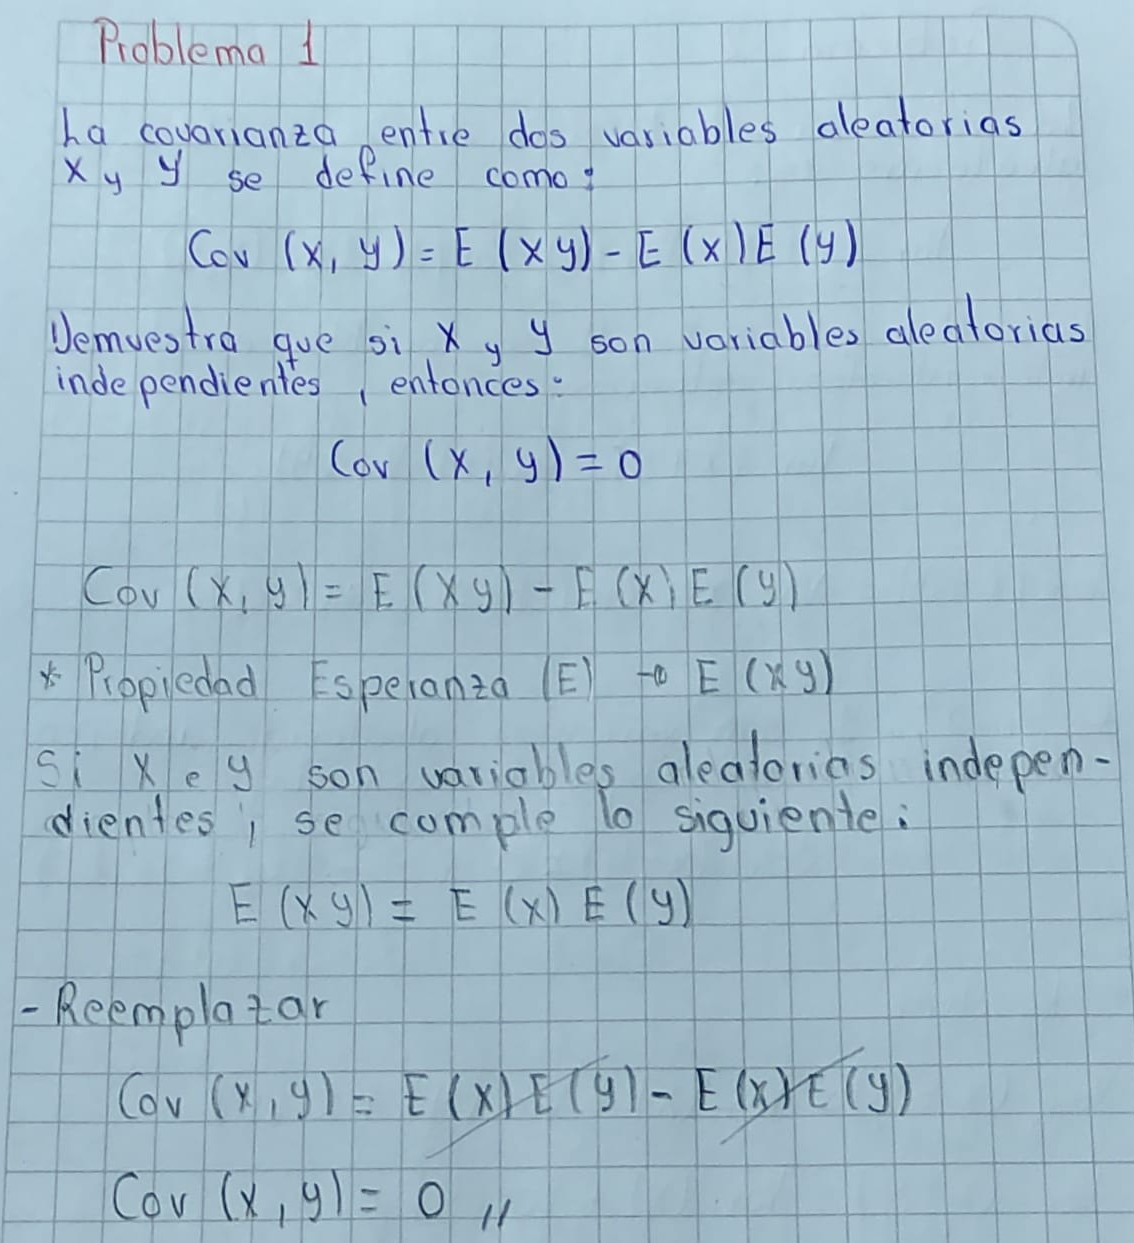
\includegraphics[width=0.581\linewidth]{/pregunta_1/1_a.jpg}
	\end{figure}


\section*{Problema 2}

La varianza de la suma de dos variables aleatorias es: 
$$Var(X+Y)=Var(X)+Var(Y)+2Cov(X,Y)$$
Demuestra que si $X$ y $Y$ son variables aleatorias independientes, entonces: 
$$Var(X+Y)=Var(X)+Var(Y)$$

\begin{figure}[H]
	\centering
	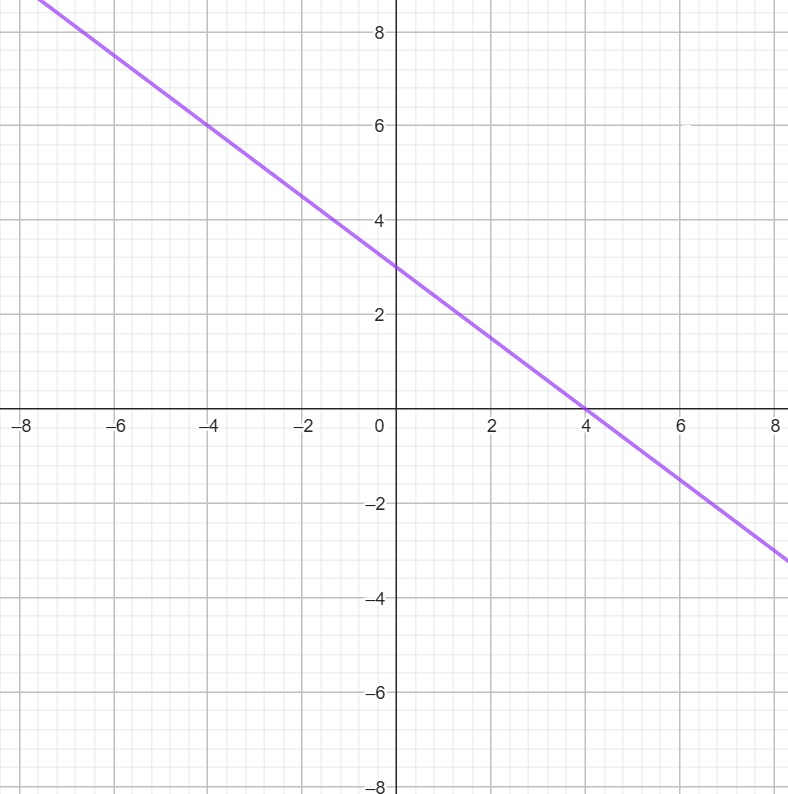
\includegraphics[width=0.92\linewidth]{/pregunta_2/2_a.jpg}
\end{figure}

\section*{Problema 3}

La varianza de una variable aleatoria $X$ se define como: 
$$Var(X)=E[(X-E(X))^2]$$
Demuestra que: 
$$E[X-E(X)]^2=E(X^2)-E(X)^2$$
Pista: Expande el término $(X-E(X))^2$ y luego calcula el valor esperado. Recuerda que $E(X)=\mu \ y \ \mu$ es un parámetro de la media poblacional y, por lo tanto, es una constante. 

\begin{figure}[H]
	\centering
	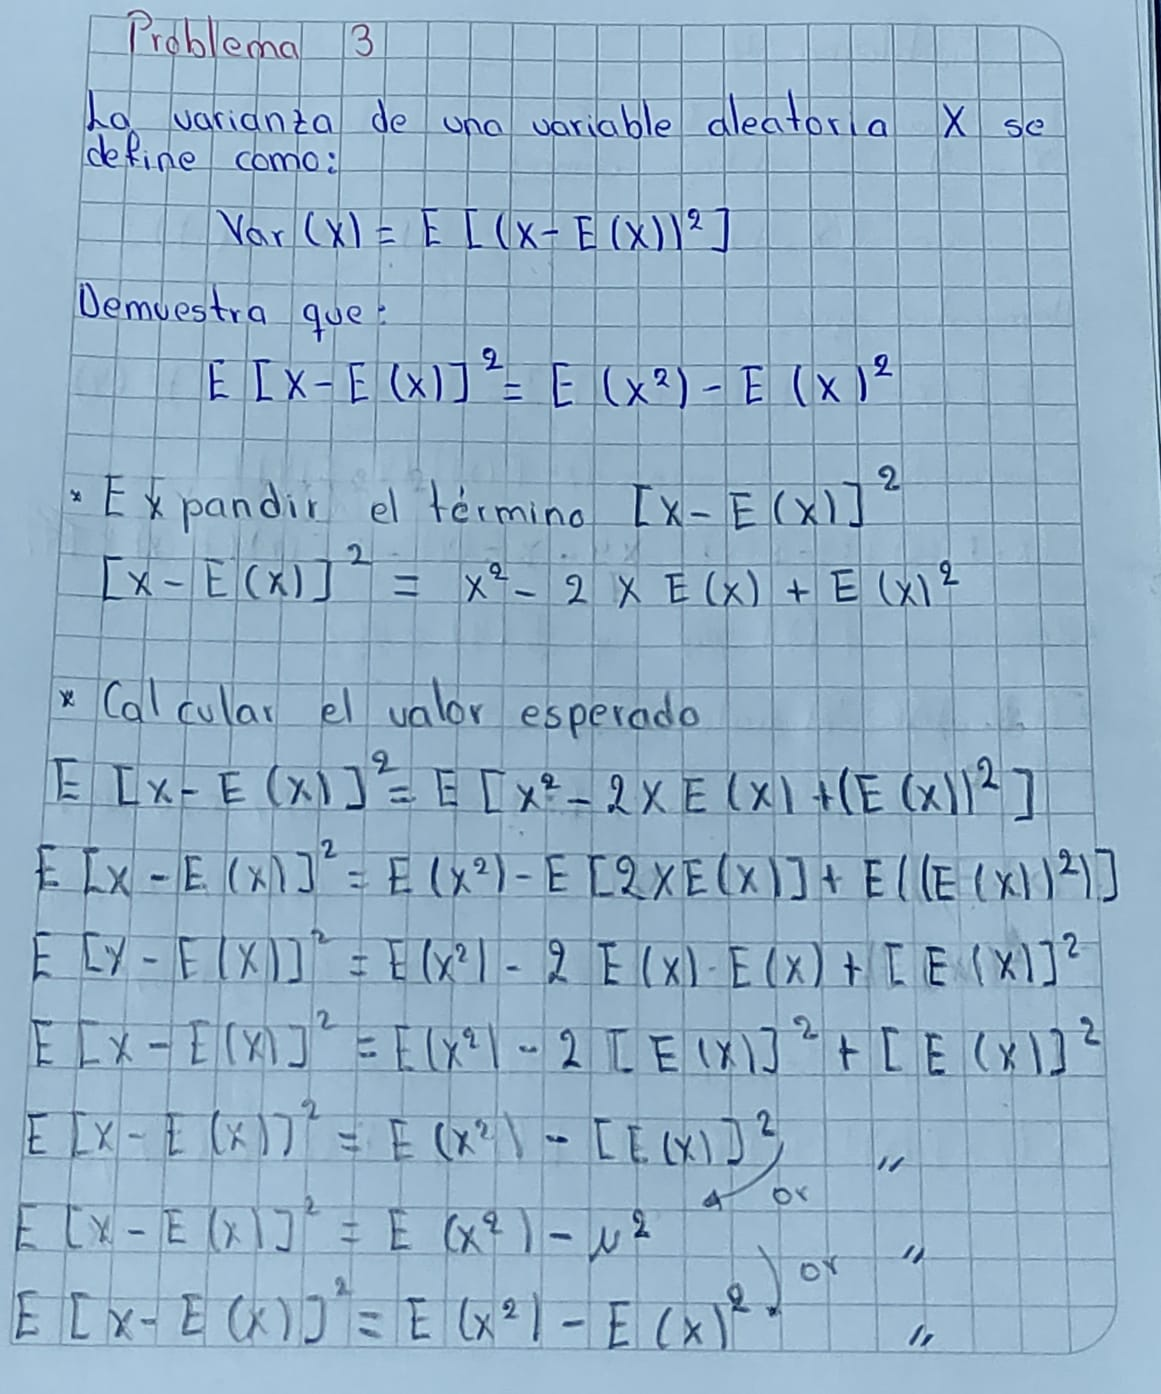
\includegraphics[width=0.84\linewidth]{/pregunta_3/3_a.jpg}
\end{figure}

\section*{Problema 4}

La covarianza entre dos variables aleatorias $X$ y $Y$ se define como:
$$Cov(X,Y)=E[(X-E(X))(Y-E(Y))]$$
Demuestra que: 
$$E[(X-E(X))(Y-E(Y))]=E(XY)-E(X)E(Y)$$
Pista: Expande el término $(X-E(X))(Y-E(Y))$ y luego calcula el valor esperado. Recuerda que $E(X)=\mu x$ y $E(Y)=\mu y$ y que $\mu x$ y $\mu y$ son parámetros y, por lo tanto, son constantes.

\begin{figure}[H]
	\centering
	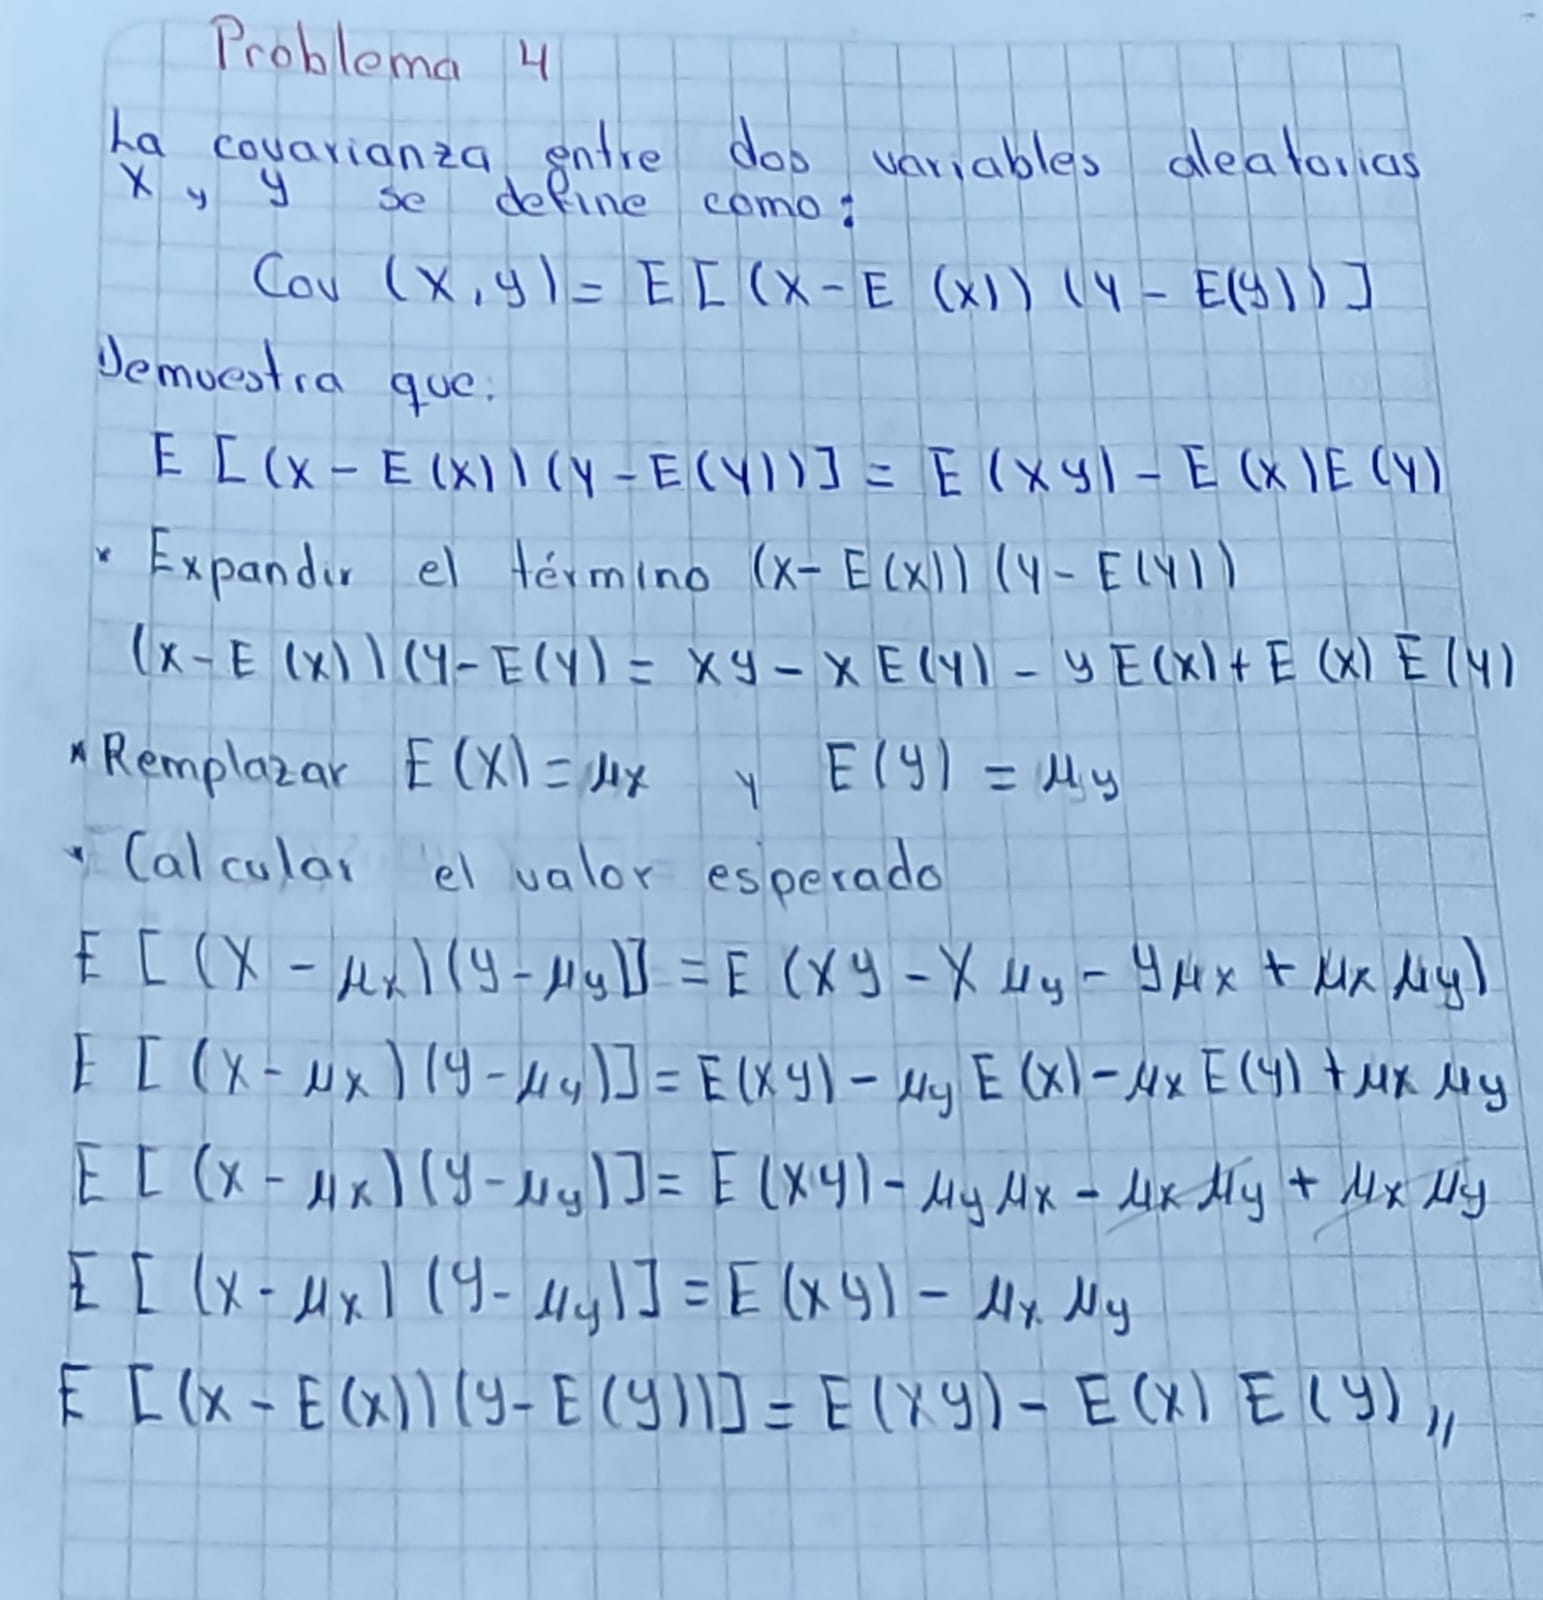
\includegraphics[width=0.95\linewidth]{/pregunta_4/4_a.jpg}
\end{figure}

\section*{Problema 5}

El estimador es insesgado si su valor esperado es igual al parámetro que se está estimando. Demuestra que la media muestra es un estimador insesgado de la media poblacional. Es decir, demuestra que: 
$$E(\bar{X})=\mu$$
donde $\bar{X}$ es la media muestral y $\mu$ es la media poblacional.
\\
Dada una muestra aleatoria $\{X_1, X_2, \ldots, X_n\}$, el estimador de la media muestral se define como: 
$$
\bar{X}	=	\frac{1}{n}	\sum_{i=1}^{n}	X_i
$$
donde $n$ es el tamaño de la muestra y $X_i$ es el valor de la variable en la i-ésima observación.

	\begin{figure}[H]
	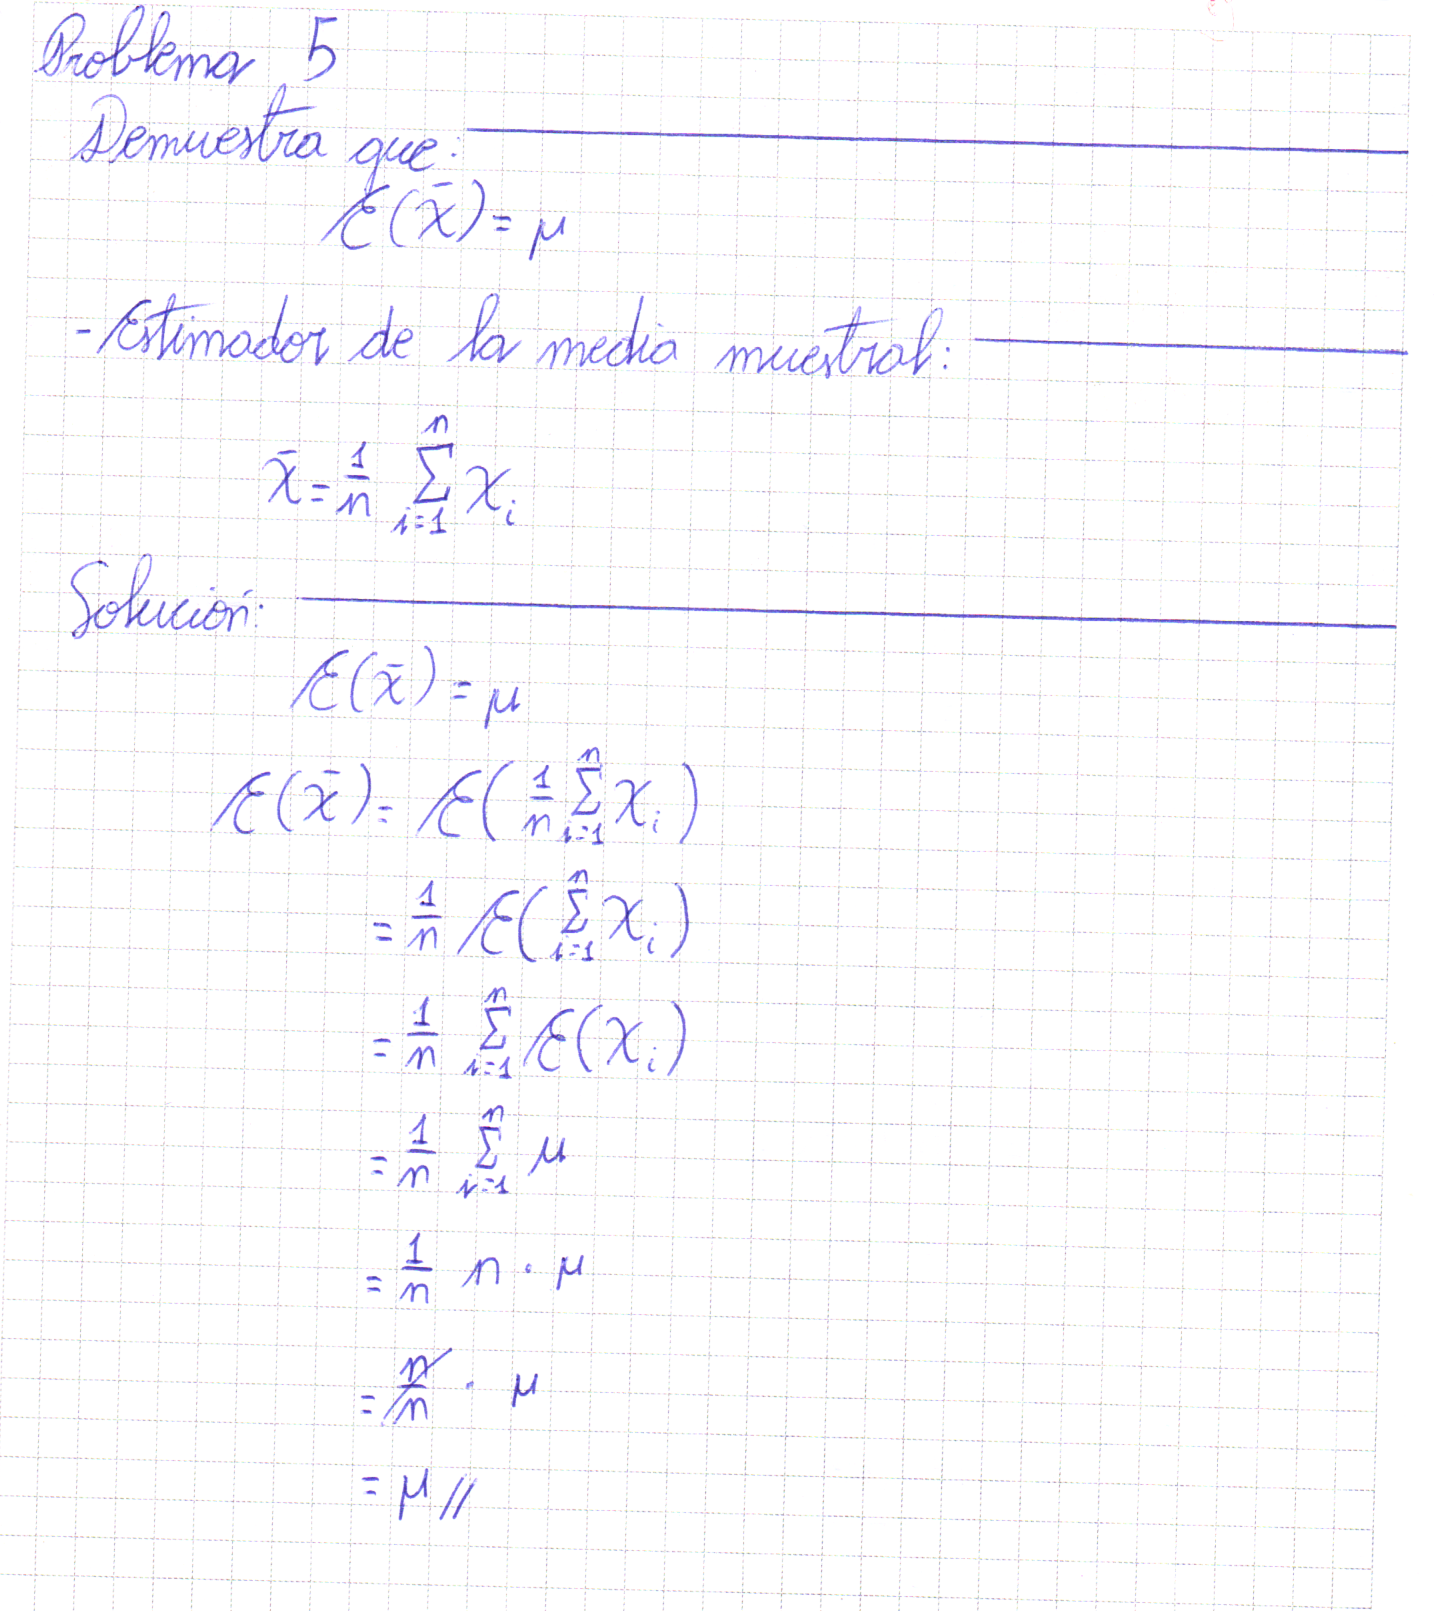
\includegraphics[width=0.86\linewidth]{/pregunta_5/5_a.png}
	\end{figure}

\section*{Problema 6}

El error estándar es una medida de la precisión de un estimador. Se define como la raíz cuadrada de la varianza del estimador. 
$$
SE(\bar{X})=\sqrt{Var(\bar{X})}
$$
Demuestra que, para la media muestral, el error estándar se define como: 
$$
SE(\bar{X})=\frac{\sigma}{\sqrt{n}}
$$
donde $\sigma^2$ es la varianza poblacional y $n$ es el tamaño de la muestra.

	\begin{figure}[H]
	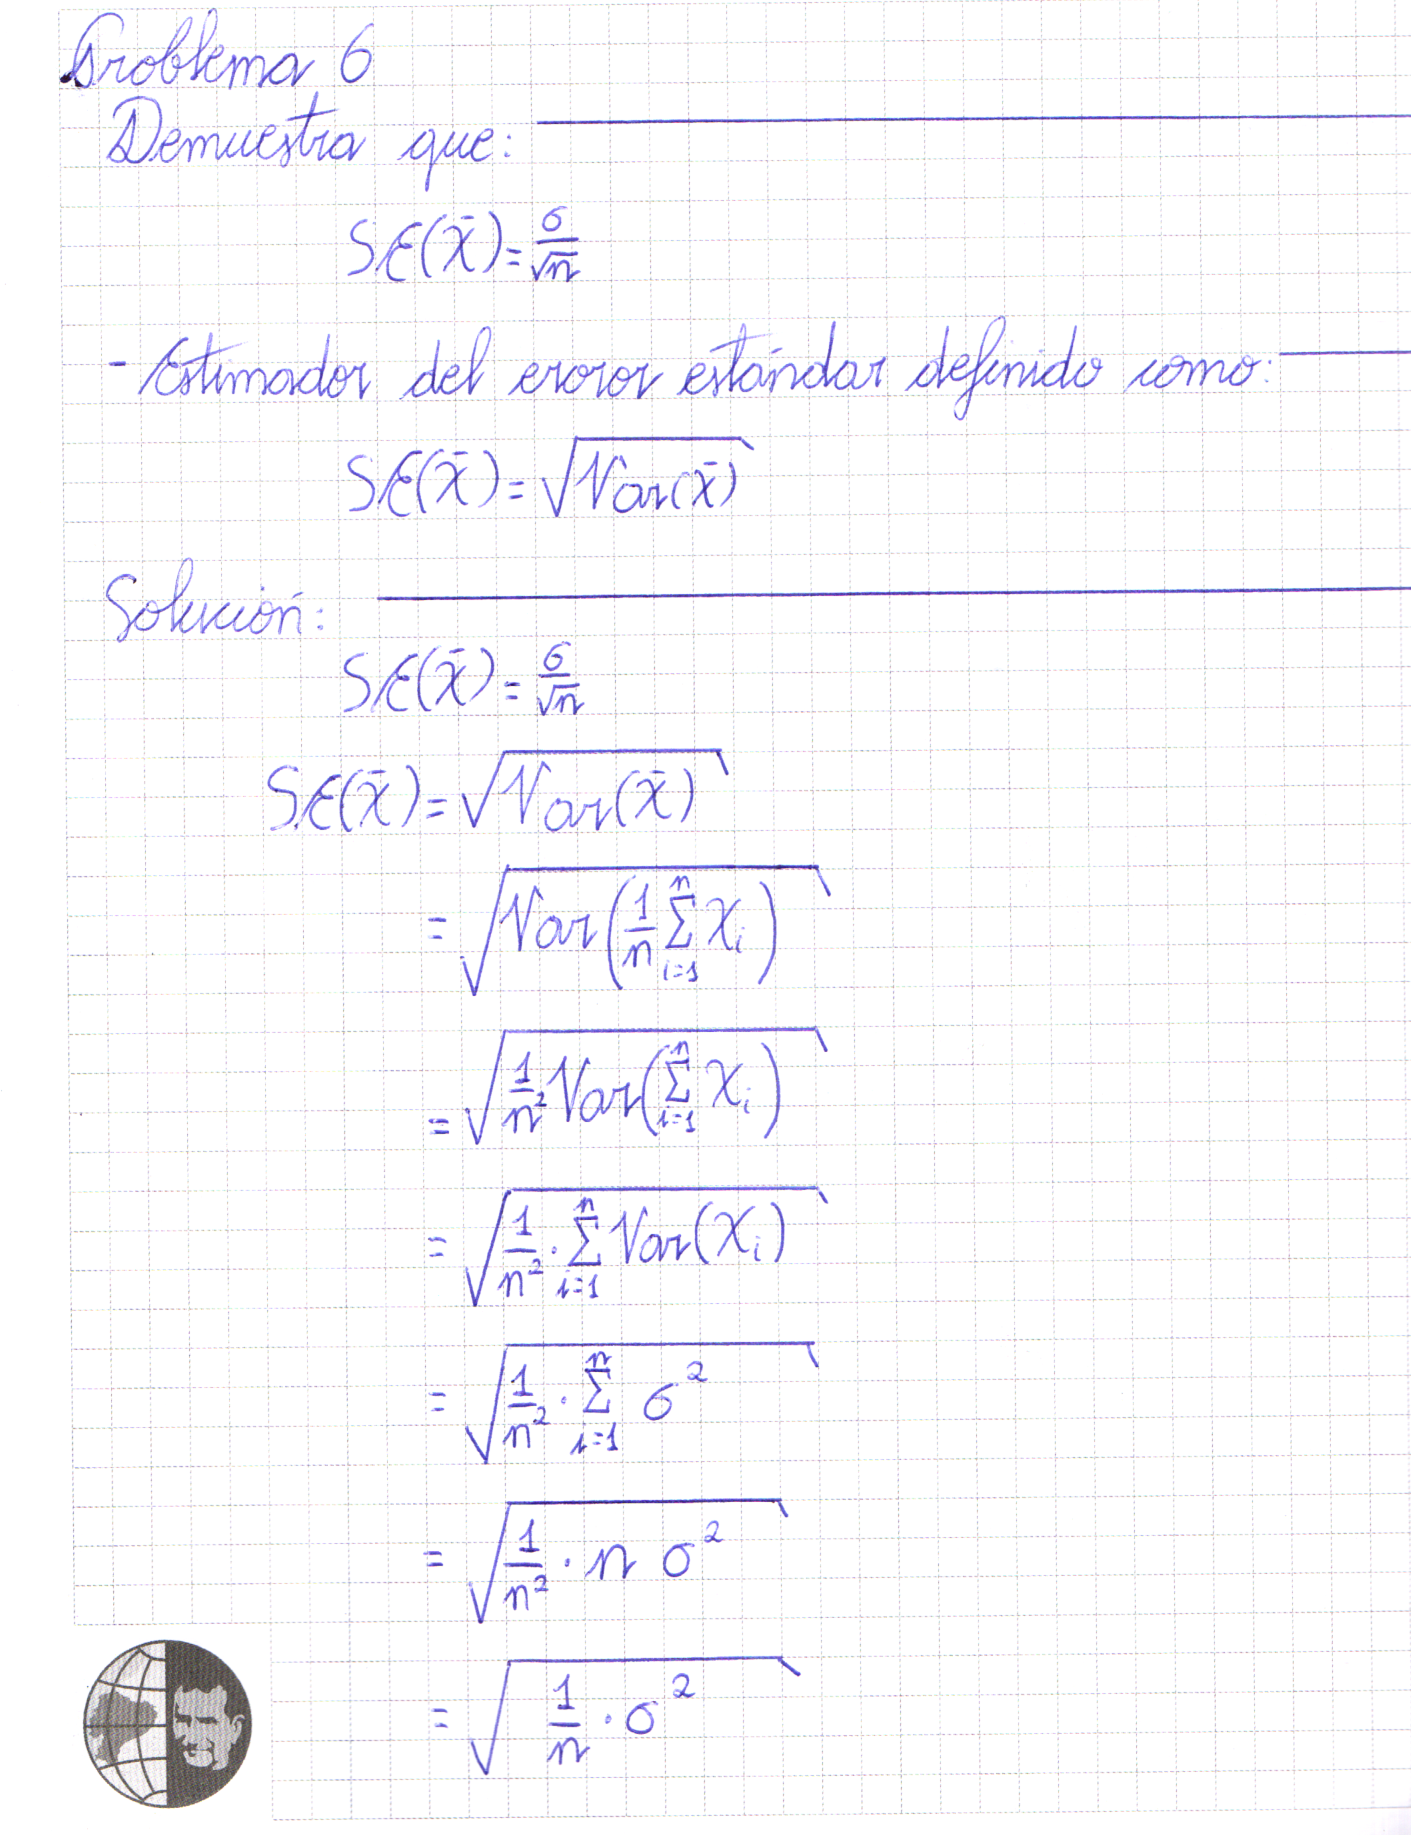
\includegraphics[width=0.7\linewidth]{/pregunta_6/6_a.png}
	\\
	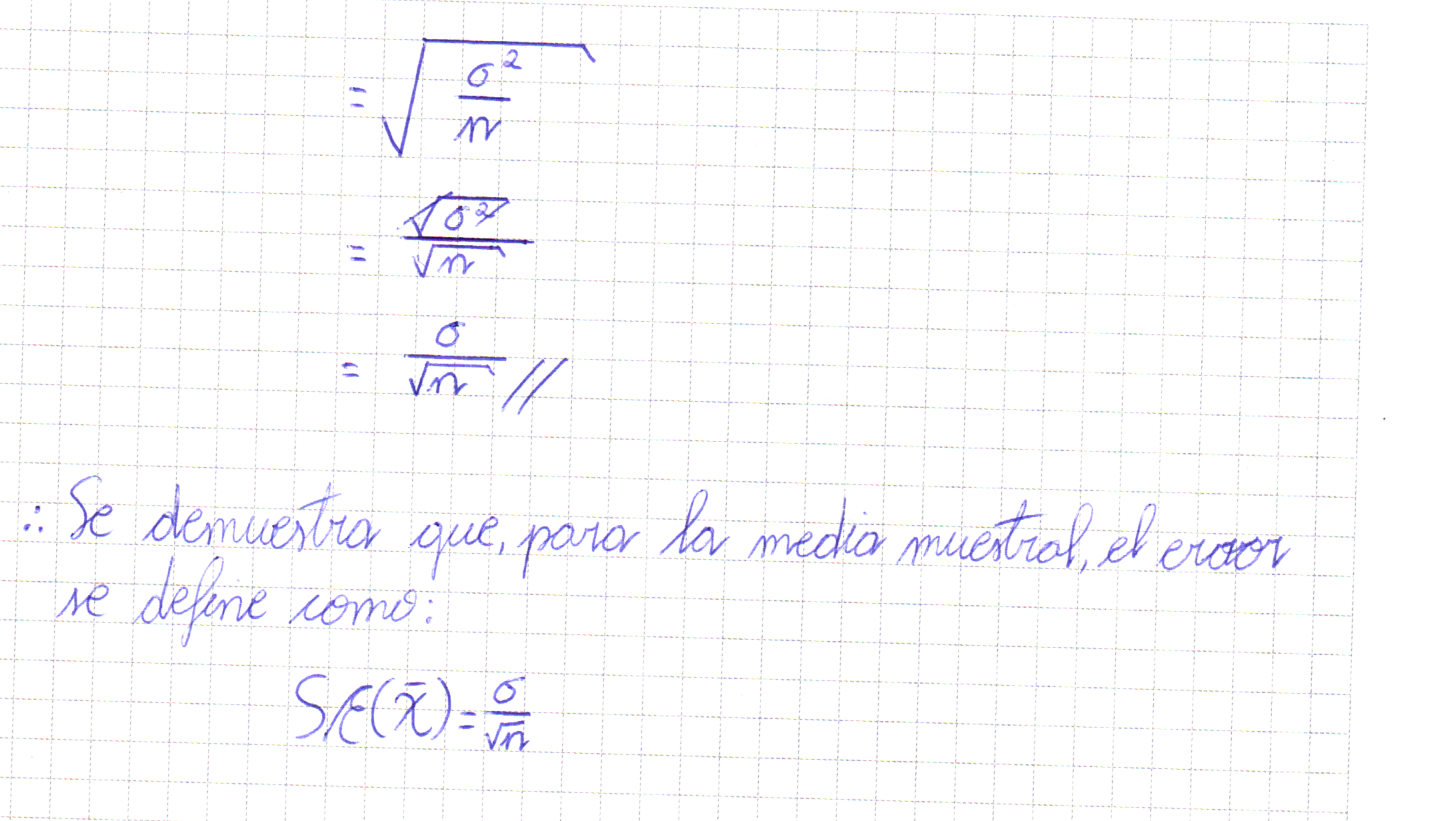
\includegraphics[width=0.86\linewidth]{/pregunta_6/6_b.png}
	\end{figure}

\section*{Problema 7}

Si alguna vez tomaron un curso de estadística en la universidad, debieron haber aprendido que la varianza de una población se calcula como: 
$$
\sigma^2=
	\frac{1}{N} 
	\sum_{i=1}^{N}
	(X_i-\mu)^2
$$
donde $N$ es el tamaño de la población, $X_i$ es el valor de la variable en la i-ésima observación y $\mu$ es la media de la población.
\\
También debieron haber aprendido que, dada una muestra aleatori $\{X_1, X_2, \ldots, X_n\}$, la varianza de una muestra se calcula como:
$$
S^2=
	\frac{1}{n-1}
	\sum_{i=1}^{n}
	(X_i-\bar{X})^2
$$
donde $n$ es el tamaño de la muestra y $\bar{X}$ es la media de la muestra. ¿Se preguntaron por qué en la varianza muestral se divide por $n-1$ y no por $n$? La razón por la cual dividimos para n-1 en lugar de $n$ es para corregir el sesgo en la estimación de la varianza poblacional.
\\
Demuestra que si tomáramos un estimador sin restar 1 en el denominador, el estimador sería sesgado. Sea $\tilde{S}^2$ el estimador de la varianza poblacional que se obtiene al dividir por $n$ en lugar de $n-1$. Demuestra que $\tilde{S}^2$ es un estimador sesgado de la varianza poblacional.
$$
\tilde{S}^2=
	\frac{1}{n}
	\sum_{i=1}^{n}	
	(X_i-\bar{X})^2
$$
Para demostrar que $\tilde{S}^2$ es un estimador sesgado de la varianza poblacional, necesitamos demostrar que el valor esperado de $\tilde{S}^2$ es diferente de $\sigma^2$. Es decir, necesitamos demostrar que
$$
E(\tilde{S}^2)\neq\sigma^2
$$
Pista: Para resolver esta ejercicio necesitarás calcular $E(X^2)$ y $E(\bar{X}^2)$. Recuerda que la varianza de una variable aleatoria $X$ se define como $Var(X)=E(X^2)-E(X)^2$. Por lo tanto, podemos despejar $E(X^2)$ como $E(X^2)=Var(X)+E(X)^2$.
\\
Igualmente, para resolver este ejercicio de forma sencilla podemos utilizar el hecho que: 
$$
\sum_{i=1}^{n} (X_i-\bar{X})^2=
	\sum_{i=1}^{n}
	X_{i}^{2}
	-
	n
	\bar{X}^2
$$ 

\begin{figure}[H]
	\centering
	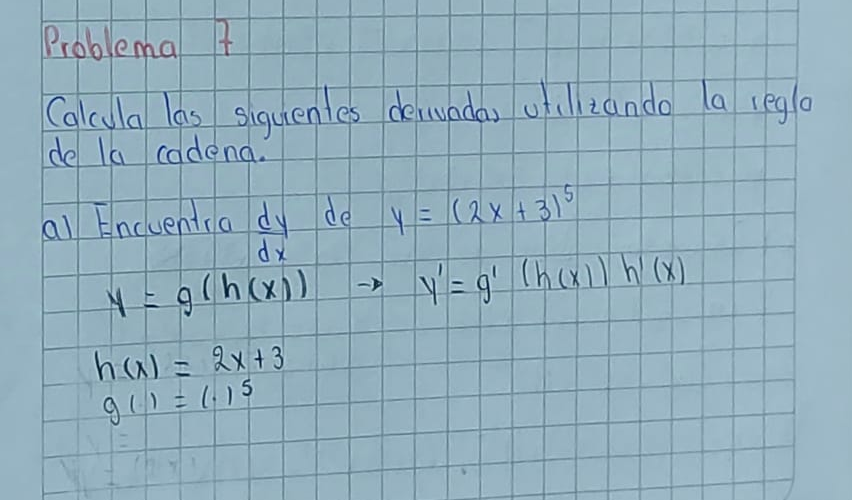
\includegraphics[width=0.64\linewidth]{/pregunta_7/7_a.png}
	\vspace{0cm}
	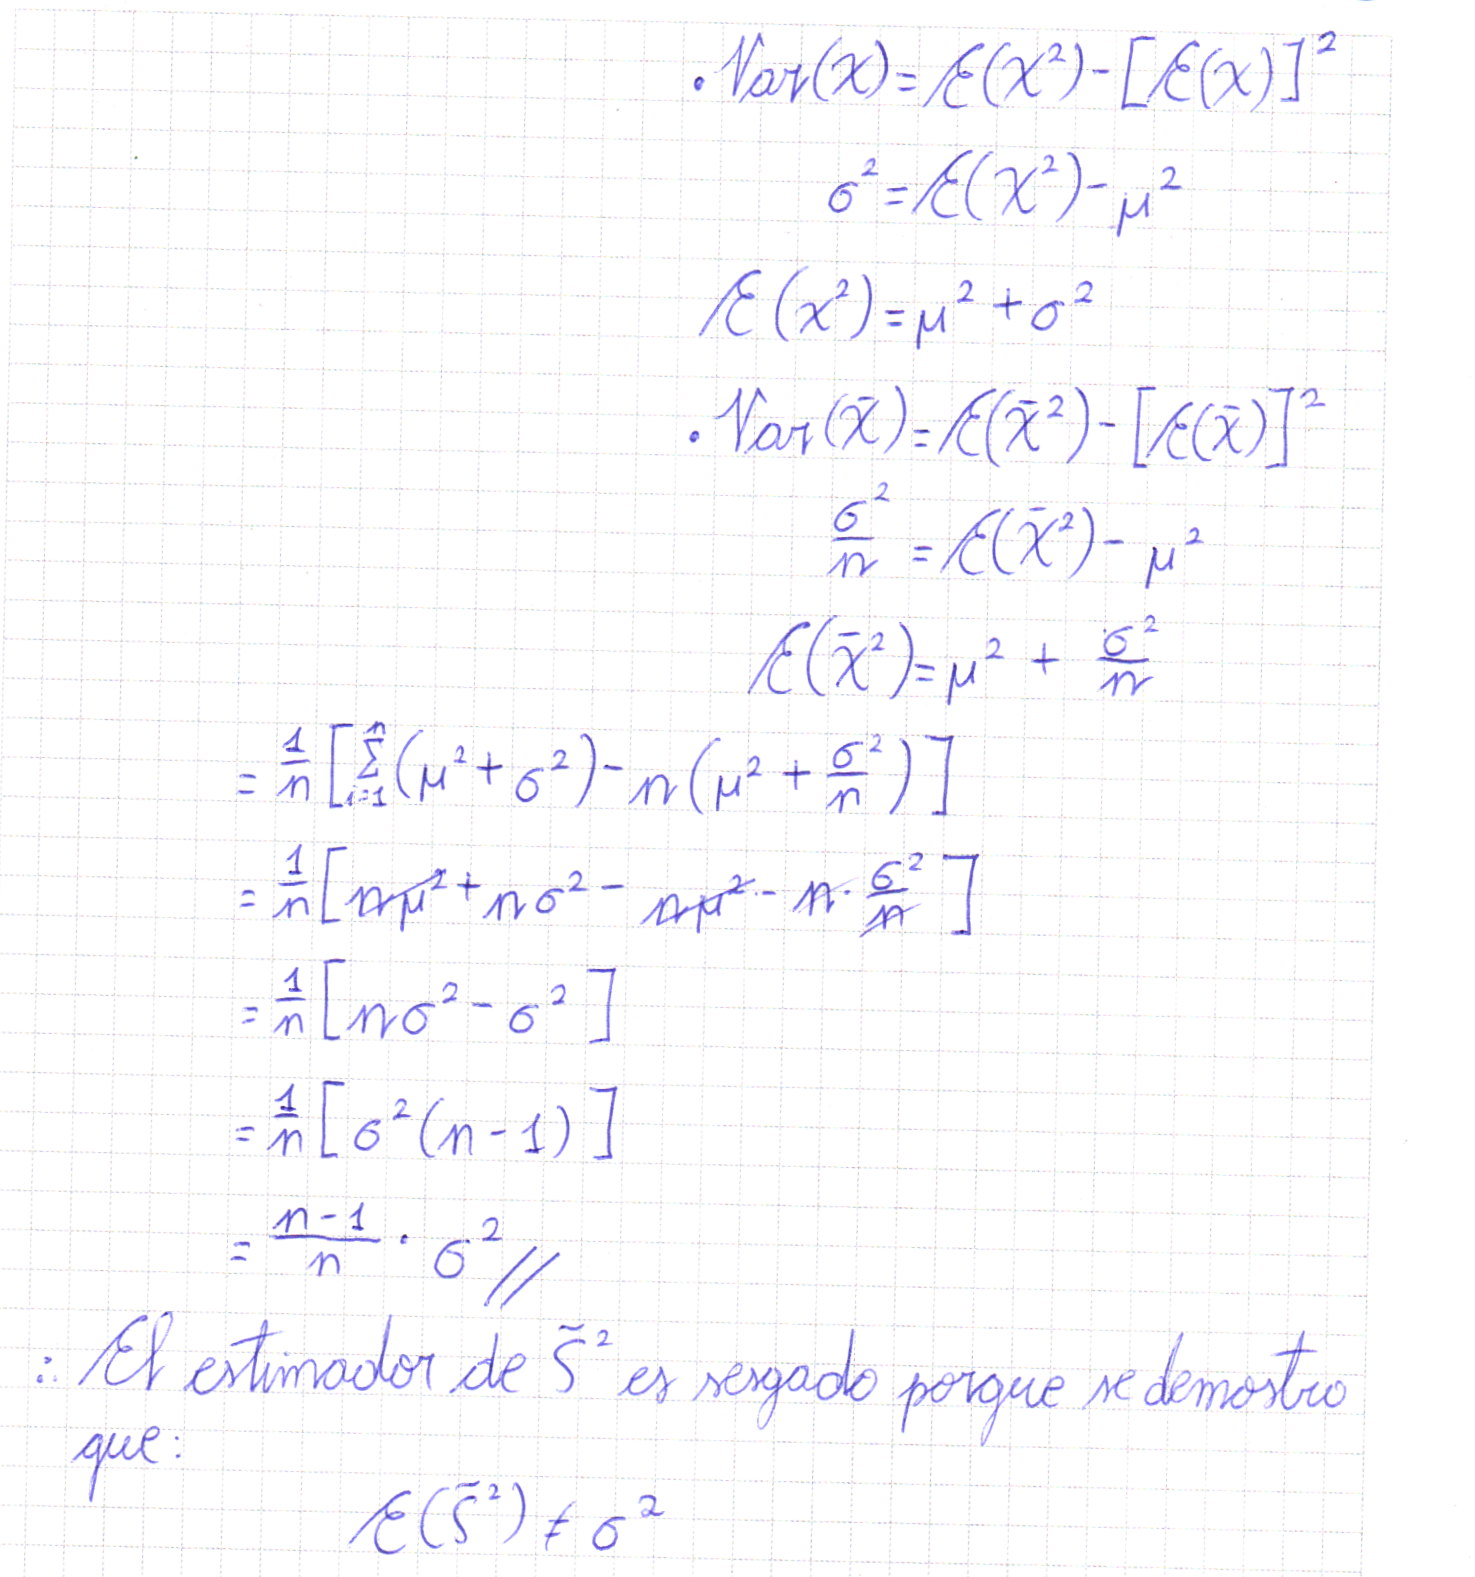
\includegraphics[width=0.64\linewidth]{/pregunta_7/7_b.png}
\end{figure}



\section*{Problema 8}

El $z-score$ o puntaje estándar es una medida estadística que indica cuántas desviaciones estándar un valor de una variable aleatoria se encuentra por encima o por debajo de la media de esa variable. Es una forma de estandarizar los datos para compararlos de manera más fácil, incluso si provienen de distribuciones diferentes o tienen escalas distintas. El $z-score$ se calcula como:
$$
Z=
\frac{X-\mu}{\sigma}
$$
donde $X$ es el valor de la variable aleatoria, $\mu$ es la media de la variable aleatoria y $\sigma$ es la desviación estándar de la variable aleatoria. 
\\
Demuestra que el valor esperado de un $z-score$ es igual a cero y su varianza es igual a uno. Es decir, demuestra que: 
$$
E(Z)=0 \ y \ Var(Z)=1
$$

\begin{figure}[H]
	\centering
	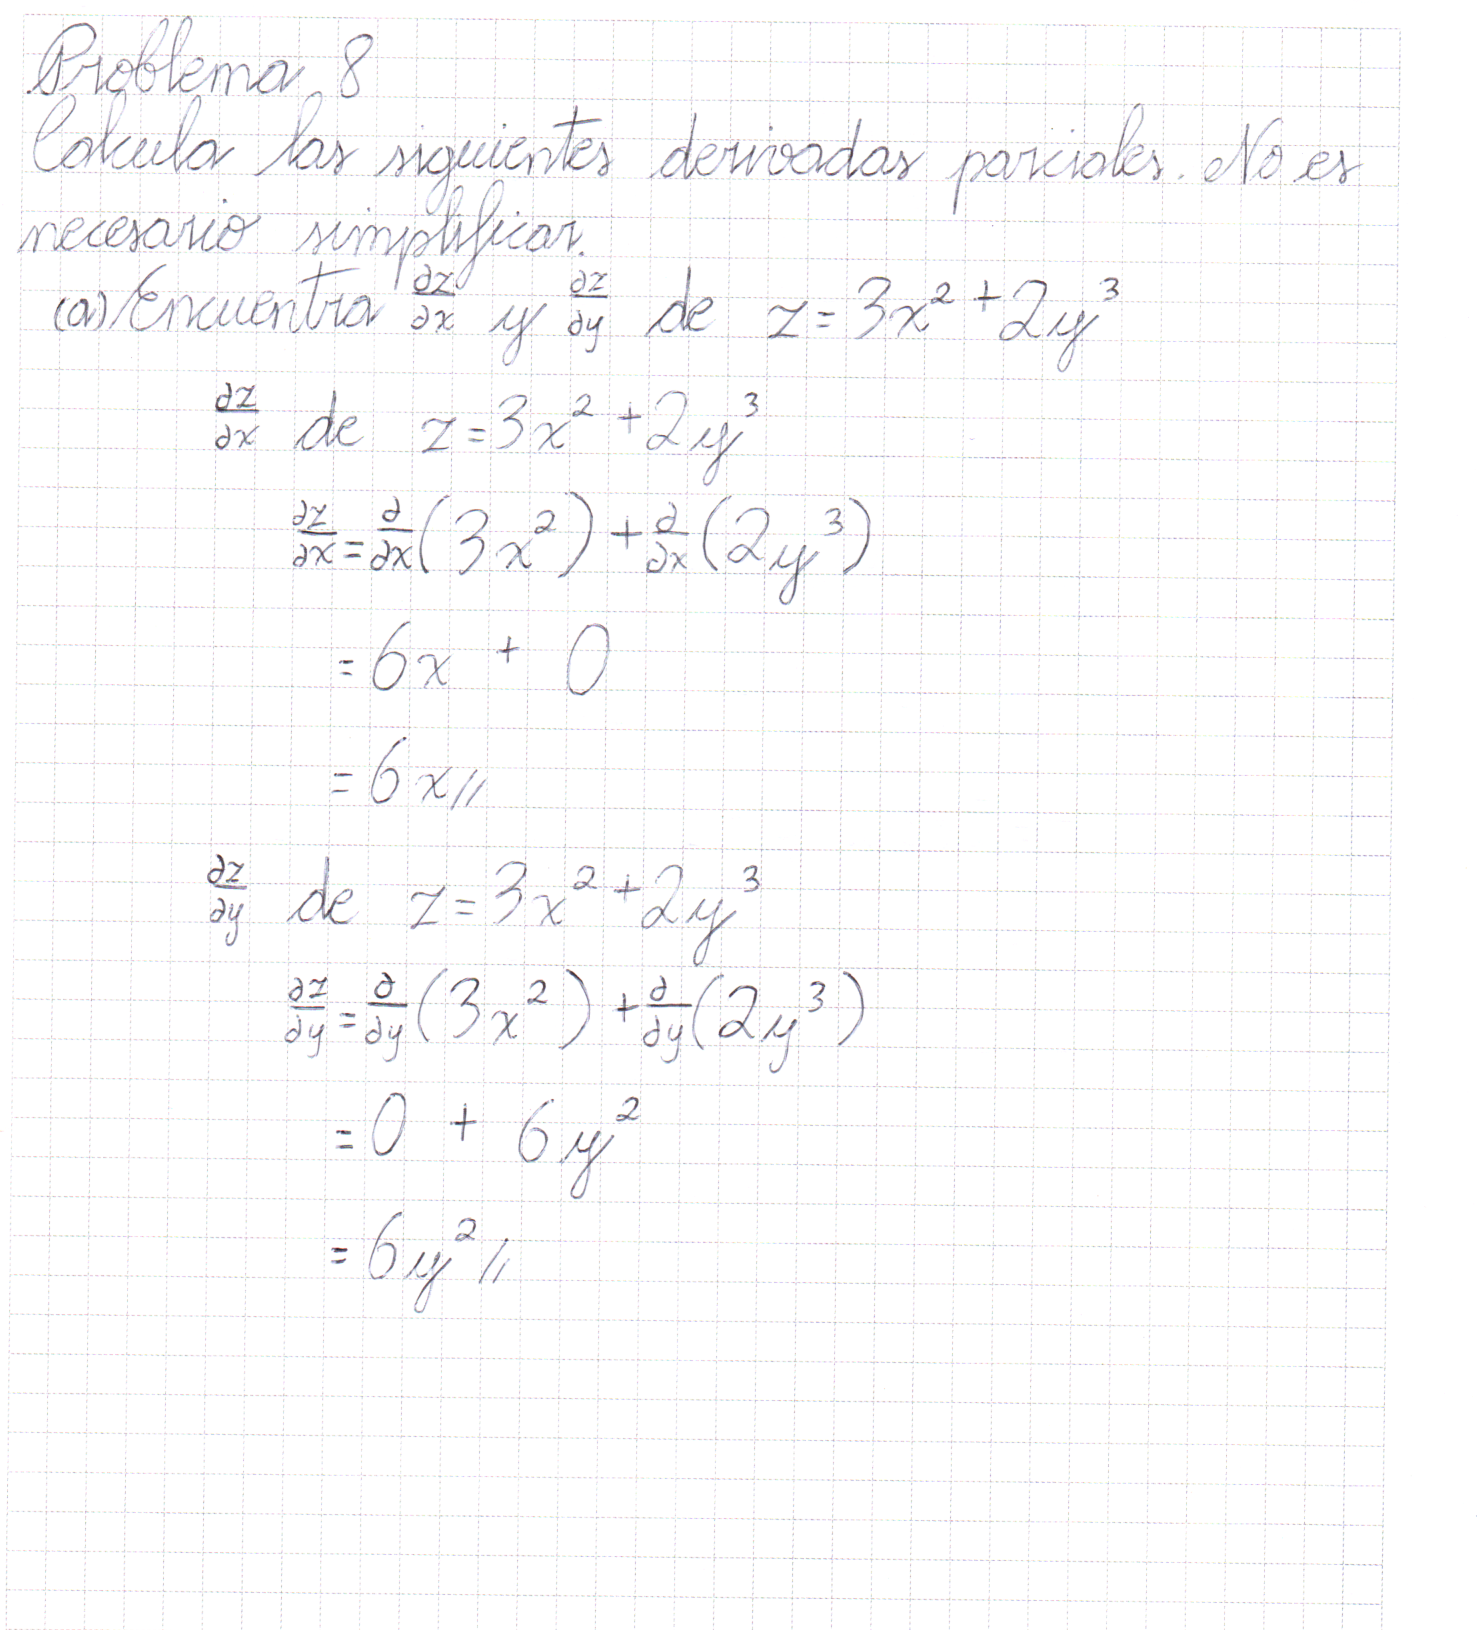
\includegraphics[width=1.1\linewidth]{/pregunta_8/8_a.png}
\end{figure}

\section*{Problema 9}

Demuestra que: 
$$
\sum_{i=1}^{n}
(X_i-\bar{X})^2
=
\sum_{i=1}^{n}
X_{i}^{2}
-
n
\bar{X}^2
$$
y que: 
$$
\sum_{i=1}^{n}
(X_i-\bar{X})
(Y_i-\bar{Y})
=
\sum_{i=1}^{n}
X_iY_i
-
n
\bar{X}
\bar{Y}
$$

\begin{figure}[H]
	\centering
	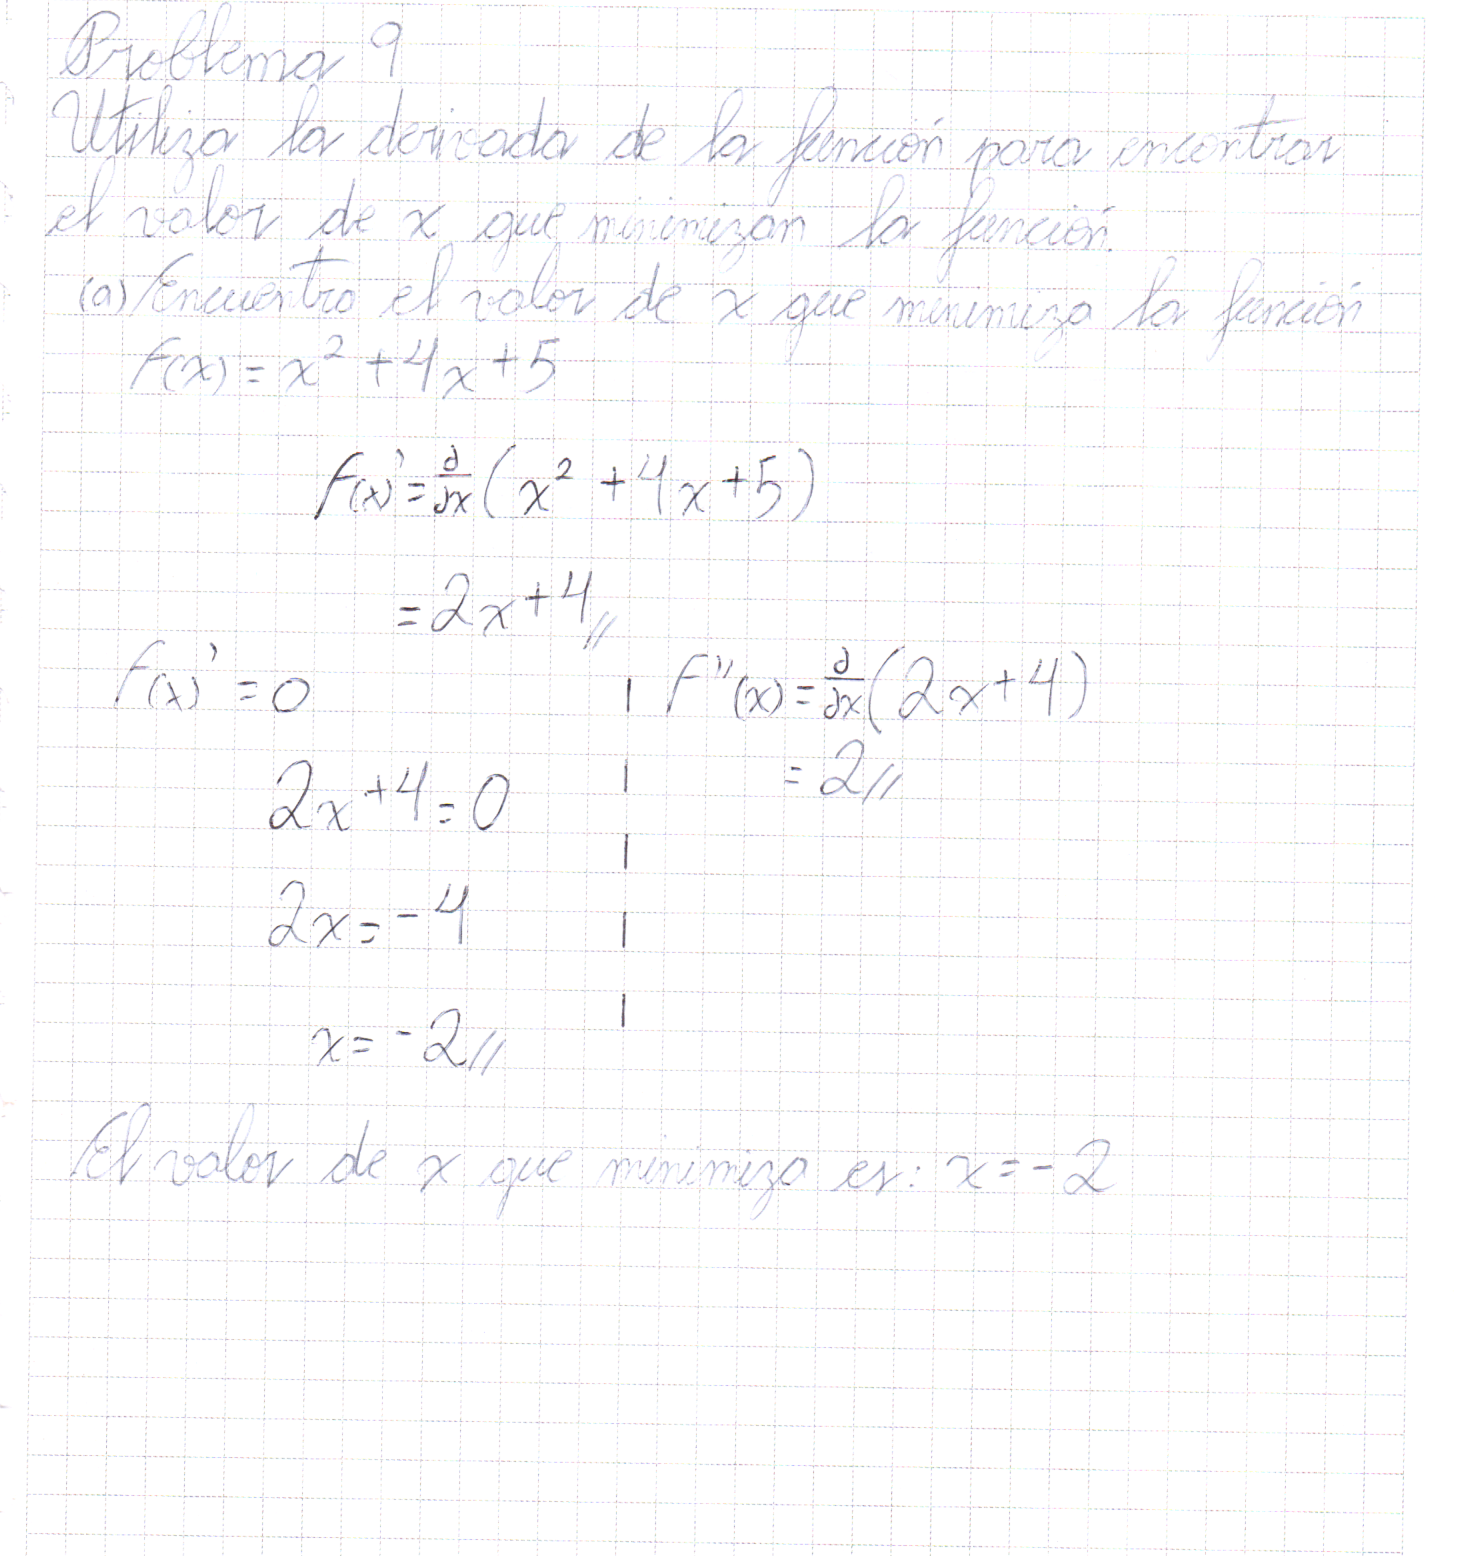
\includegraphics[width=1.1\linewidth]{/pregunta_9/9_a.png}
\end{figure}

\newpage

\section*{Problema 10}

Dada una muestra aleatoria
$\{(X_i, Y_2): n=1,2,\ldots,n\}$, el modelo de regresión lineal simple se define como:
$$
Y_i=
	\beta_0
	+
	\beta_1X_i
	+
	u_i
$$
donde $\beta_0$ y $\beta_1$ son los coeficientes de la regresión y $u_i$ es el término de error. Utilizando el método de mínimos cuadrados, demuestra que los estimadores de los coeficientes de la regresión son:
$$
\hat{\beta_0}=\bar{Y}-\hat{\beta_1}\bar{X}
$$
$$
\hat{\beta_1}
=
\frac
{
	\sum_{i=1}^{n}
	(X_i-\bar{X})
	(Y_i-\bar{Y})
}
{
	\sum_{i=1}^{n}
	(X_i-\bar{X})^2
}
$$

\begin{figure}[H]
	\centering
	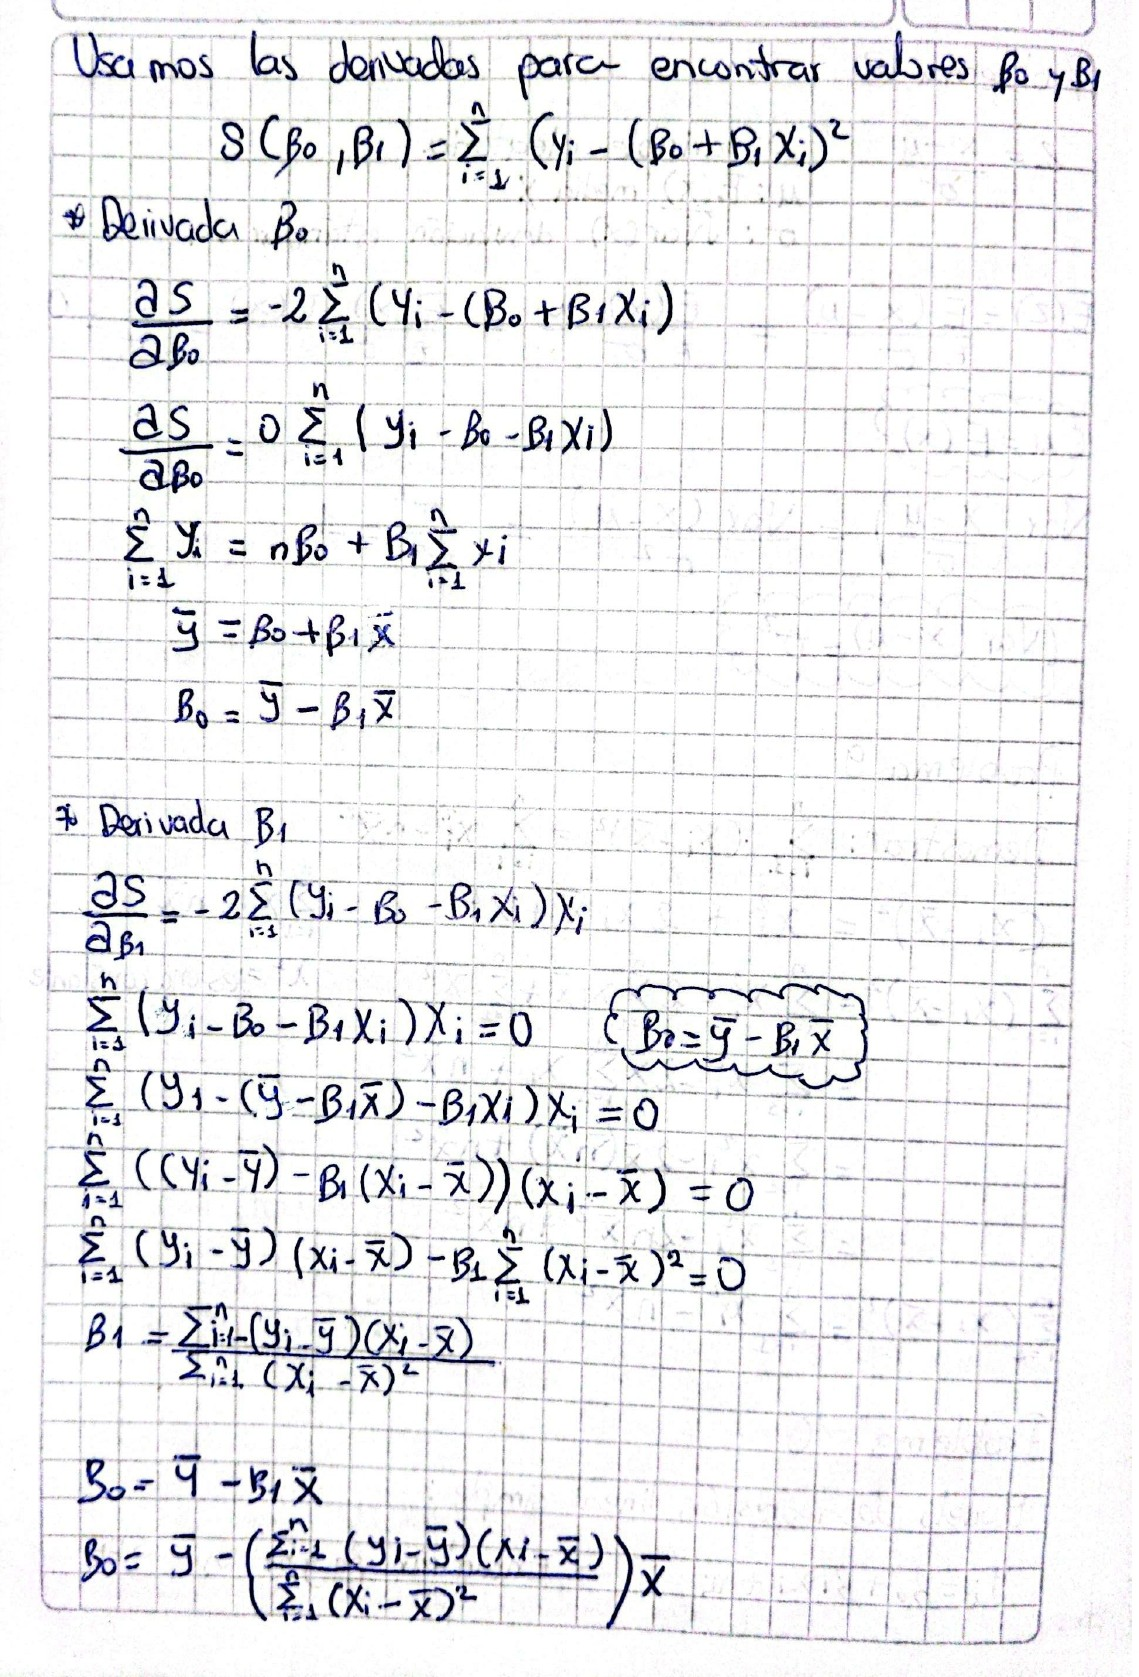
\includegraphics[width=0.64\linewidth]{/pregunta_10/10_a.jpg}
\end{figure}


\end{document}
